%*----------- SLIDE -------------------------------------------------------------
\begin{frame}[t]{Determinante} 

    O determinante permite verificar se uma matriz possui uma inversa ou não. Caso o determinante da matriz seja \textbf{diferente} de zero, a matriz possui uma inversa.

    \vspace*{0.3cm}

    \begin{equation}
        \det\begin{pmatrix}
            3 & 0 \\
            0 & 2 \\
        \end{pmatrix}
        =
        3*2-0*0
        =
        6
    \end{equation}

    \vspace*{0.3cm}

    \begin{columns}[c]
        \column{.4\textwidth}
        \hspace*{0.0cm}
        \centering
        O cálculo do determinante envolve a regra de \textbf{Sarrus}.
       \column{.6\textwidth}
       \centering
       \begin{figure}
        
\includegraphics[width=0.6\textwidth]{sarrus_rule.png}
    \end{figure}
   \end{columns}
%*----------- notes
    \note[item]{Notes can help you to remember important information. Turn on the notes option.}
\end{frame}
%-

%*----------- SLIDE -------------------------------------------------------------
\begin{frame}[t]{Sistemas de equações lineares} 

   Um dos problemas mais importantes na matemática é o da resolução de um \textbf{sistema de equações lineares}. 
   
   De acordo com \cite{leon2000algebra}, mais de 75\% de todos os problemas matemáticos encontrados em aplicações científicas e industriais envolvem a resolução de um sistema linear em algum estágio.

   \vspace*{0.45cm}

   \centering

   $a_{1}x+{1} + a_{2}x+{2} + a_{n}x+{n} = b$

   $a_{1}x+{1} + a_{2}x+{2} + a_{n}x+{n} = b$

   .

   .

   .

   $a_{1}x+{1} + a_{2}x+{2} + a_{n}x+{n} = b$

%*----------- notes
    \note[item]{Notes can help you to remember important information. Turn on the notes option.}
\end{frame}
%-
%*----------- SLIDE -------------------------------------------------------------
\begin{frame}[t]{Mínimos Quadrados} 

    O ajuste por mínimos quadrados é uma técnica de otimização matemática que busca \textbf{minimizar} a soma dos quadrados das diferenças entre o valor estimado e os dados observados.
 
    \vspace*{0.45cm}
 
\begin{columns}[c]
    \column{.5\textwidth}
    % \hspace*{0.9cm}
    \centering
    A técnica dos mínimos quadrados foi desenvolvida independentemente por \textbf{Adrien-Marie Legendre} e \textbf{Carl Friendrich Gauss}.
   \column{.5\textwidth}
   \centering
   \begin{figure}
    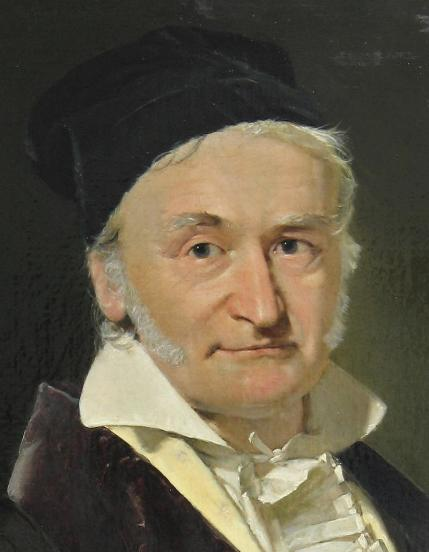
\includegraphics[width=0.4\textwidth]{gauss.png}
    \caption{Retrato de Gauss}
    \end{figure}
\end{columns}

 %*----------- notes
     \note[item]{Notes can help you to remember important information. Turn on the notes option.}
 \end{frame}
 %-